\documentclass[]{article}

\usepackage[french]{babel}
\usepackage[T1]{fontenc}
\usepackage{titlesec}
\usepackage[top=2.5cm, bottom=2cm, left=3cm, right=3cm]{geometry}
\usepackage{lmodern}
\usepackage[latin1]{inputenc}
\usepackage{graphicx}
\usepackage{caption}
\usepackage{subcaption}
\usepackage{mathpazo}
\usepackage{amssymb,amsmath}
\usepackage[protrusion=true,expansion=true]{microtype}

%opening
\title{
\huge{\textbf{{Financial Product Report}}}\\
\bigskip
\large{\textsc{Expert version}}
}
\author{Paul-�mile \textsc{Buteau} (81323850), Julien \textsc{Wissocq} (81323847)}

\begin{document}

\maketitle


\section{Introduction}

This report presents the result of the simulation which has been done about the financial product sold by Daiwa Securities. The aim of the simulation is to decide if it is valuable to invest in this financial product. The mean value and the variance of return of this product has been evaluated to answer this question.
The financial product has the following properties:

\subsection{Market Prices}
This financial product follows the evolution of two different market prices: the Standard \& Poor's 500 and the Nikkei 225.
At the starting day of contract related to the financial product, the value of each of these market prices are used as the reference value which represents 100\%.

\subsection{Interest Rate}
The interest rate is 3\% per year. Because the payment of the interest is done twice per year, the bi-annual interest rate is then 1.5\%.
The market prices are evaluated 10 days before the payment day. We will refer to those days as evaluation days.
This interest rate is fixed over the maturity time of the product.

\subsection{Knock-In}
The knock-in value is set to 60\%. During the 3 years of lifespan of the product, if the value of ANY of the followed market prices drops down to 60\% of its referential (or initial) value, the knock-in is activated.
The knock-in status is evaluated at every business day and not only at the evaluation days.
The consequences of this activation will be presented in the repayment cases section.

\subsection{Knock-Out}
The knock-out value is set to 105\%. During the 3 years of lifespan of the product, if the value of BOTH followed market prices reach to 60\% of its referential (or initial) value, the knock-in is activated.
Unlike the knock-in, the knock-out status is evaluated only on evaluation days.
If the knock-out is activated, the financial product becomes out of date. However, the next payment day is still due to the investor.

\newpage

\subsection{Repayment cases}
Depending on the evolution of the market prices, we have to consider 4 different repayment cases. They are presented in the following table:

\begin{table}[h]
	\centering
	\begin{tabular}{|c|c|c|c|} 
    \hline
    \multicolumn{2}{|c|}{Repayment rate} & \multicolumn{2}{c|}{Knock-in} 										 \\
		\cline{3-4}
    \multicolumn{2}{|c|}{}  						 & Not activated 	& Activated 											 \\
    \hline
		Knock-out & Not activated 					 & 1 							& $min(\frac{S_{j,T}}{S_{j,0}},1)$ \\
		\cline{2-4}
							& Activated 							 & 1 							&	1 															 \\
    \hline
	\end{tabular}
	\caption{The different rates of repayment cases, depending on realization of knock-in and knock-out}
\end{table}


\section{Details of the simulation}

The following section presents the theoretical aspects that has been thought to realize the evaluation of the financial product sold by Daiwan Securities. However, the details about the implementation realized using Java language will not be presented in this report for convenience.

\subsection{Generation of the Market Prices}

In order to get an estimation of the mean and variance of our financial product return, we need to simulate the behavior of S\&P and Nikkei market prices. Because a market price has an extremely complex behavior, we need to model its evolution.

\subsubsection{Geometrical Brownian Motion}

The geometrical Brownian motion process has been chosen for modeling the market prices evolution. The recurrence formula for the geometrical Brownian motion is:

\begin{gather*}
	S_j(t+\Delta t) = S_j(t) \;
		e^{\bigl(\mu_j-\frac{{\sigma_j}^2}{2}\bigr)\Delta t+\sigma_j \sqrt{\Delta t}\xi_j}
\end{gather*}

\bigskip

with the following terminology:
	\begin{itemize}
		\item S is the closing price of an index% (either S\&P500 or Nikkei225)
		\item $\Delta t$ is the constant time step%, expressed in years ($\approx \frac{1}{252}$) 
		\item $\mu$ is the mean of the log return of an index price
		\item $\sigma$ is the volatility
		\item $\xi$ is the independent standard normal distribution
	\end{itemize}

\bigskip

In order to generate a correct path for the market prices, we need mainly to estimate the volatility of the two market prices.

\subsubsection{Estimation of the volatility}

The volatility has been estimated using the last 3 months historical data of both market prices. According to the HULL, the volatility should be estimated using the last 3 or 6 months of historical data, older data is considered as irrelevant. The volatility have been estimated using the following formula:

\[
\hat{\sigma}_j = \sqrt{\frac{1}{m-1} \sum_{i=1}^m (u_{j,i}-\hat{\mu_j})^2}
\]

\bigskip

where $\mu_j$ is the mean value of the log return which can be considered as zero.
The following values has been found: $\sigma_{S\&P} = 23 \%$ and $\sigma_{Nikkei} = 43 \%$

For simplicity, we decided to not reestimate the volatility during the simulation.

\subsection{Monte Carlo method}

For this simulation, we decided to use only the standard Monte Carlo method for simplicity.

\section{Results of the simulation}

\subsection{Market Price generation}

Using the geometrical Brownian motion, we are able to generate different paths for the market prices. The following figure presents one of the possible path that can appear. We only generate new closing prices on business days which excludes week-ends and holidays.

\bigskip

\begin{figure}[h!]
\centering
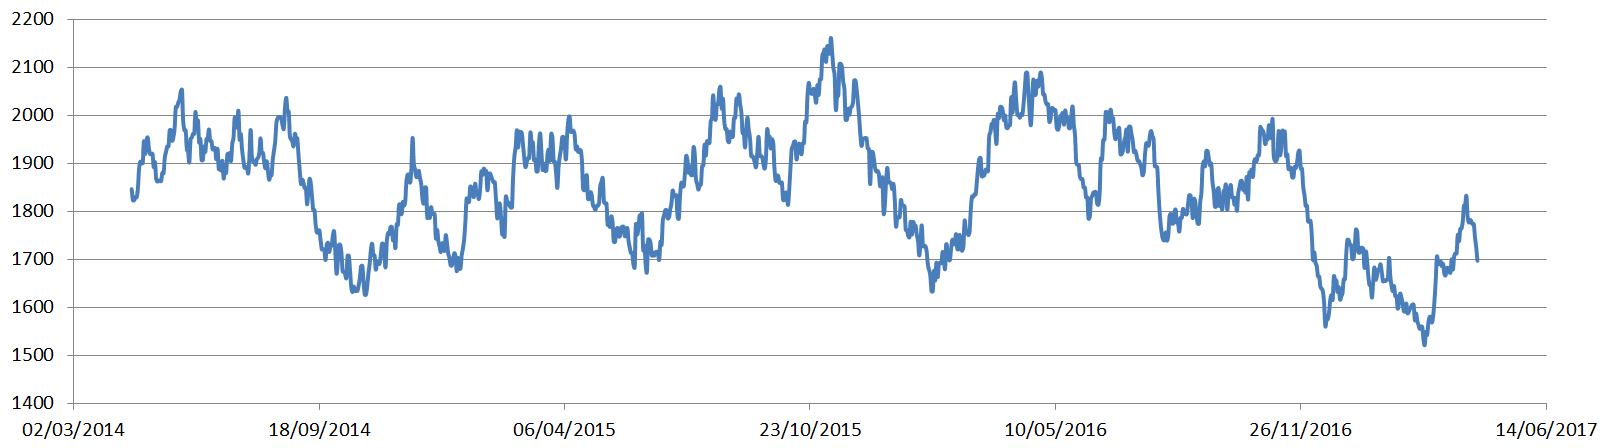
\includegraphics[width=10cm]{SandP500_simulated}
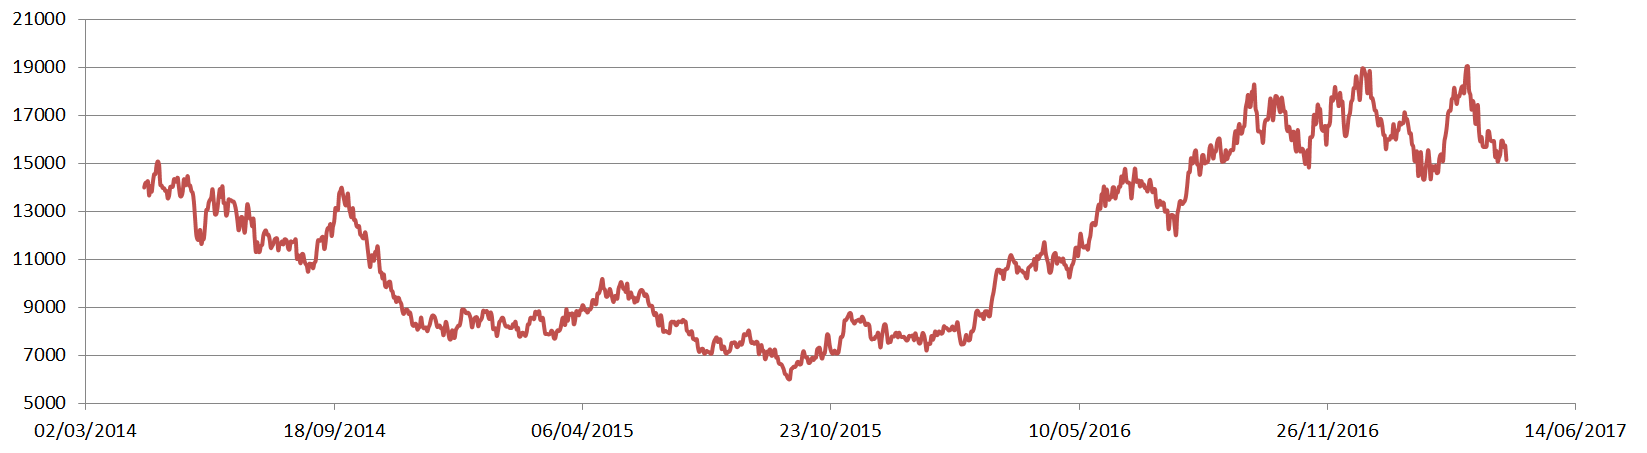
\includegraphics[width=10cm]{Nikkei225_simulated}
\caption{S\&P (top) and Nikkei (bottom) possible path over 3 years}
\end{figure}



\subsection{Monte Carlo method results}

\subsubsection{Mean \& standard deviation of the financial product return}

On every business day, we evaluate if a knock-in appears. On each evaluation day, we add the interest to the gain which had been set to -1 to take into account the first investment. On each evaluation day, we also evaluate if the knock-out appears. If it is the case, we stop the future evaluation, add the last interest payment due and retrieve the total amount invested (+1).

After the 3 years, if the knock-in has been activated during the simulation, we calculate the final repayment of the first interest according to the formula in the table 1.
For this simulation, we took a number of sample equals to 10,000. The simulation duration is about 10 seconds. We found the following results:

\bigskip

\begin{itemize}
\item Mean value of the return: -26.1\%
\item Standard deviation of the return: 8.9\%
\end{itemize}

\newpage

\subsubsection{Cumulative density function of the return}
The figure 2 presents the cumulative density function (CDF) of the return of the financial product. It gives the probability for a specific return to appear.

\begin{figure}[h!]
\centering
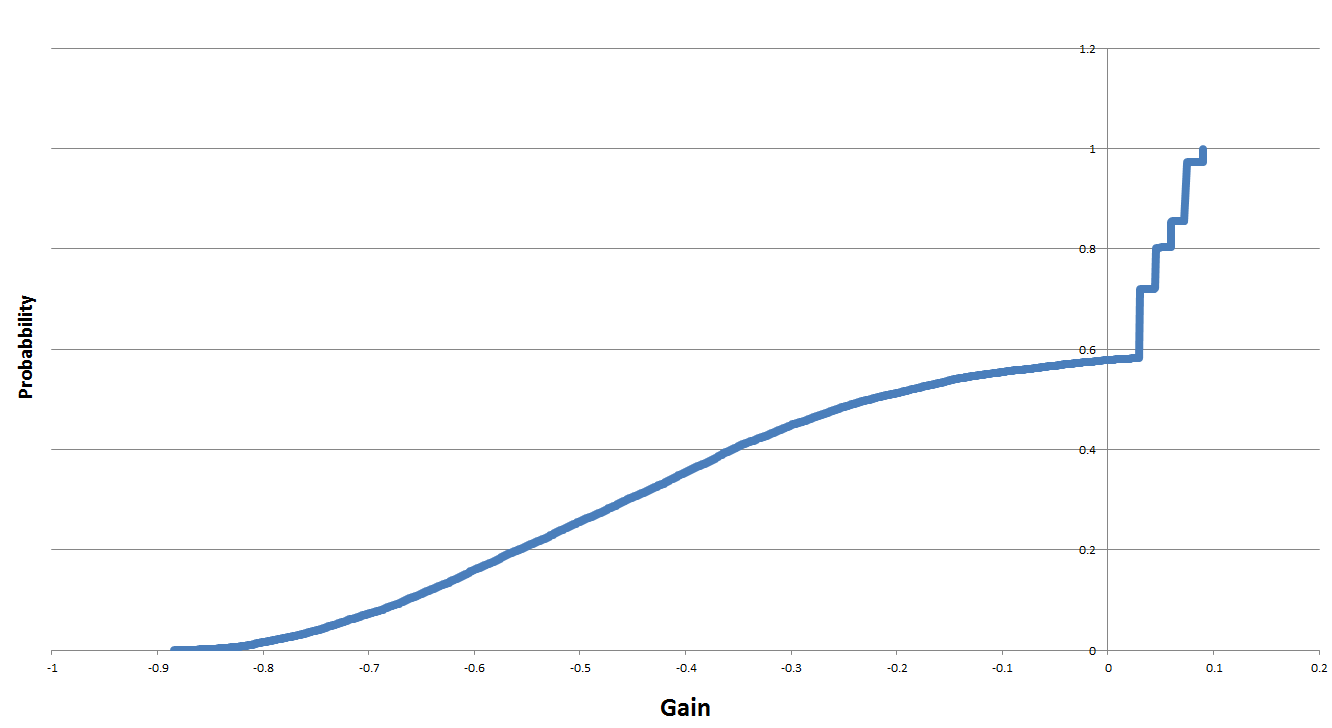
\includegraphics[width=10cm]{Gain}
\caption{Cumulative density function of the return}
\end{figure}

As we can see on this figure, the probability to have a gain with this financial product is about 40\% for a gain which cannot go over 9\% of the investment. On the other hand, the probability of loss is about 60\% for a loss that can reach 90\% (theoretically 100\%) of the investment.

\subsection{Conclusion of the simulation}
According to the above results, it is clear that this financial product is not valuable for an investment for many reasons:

\begin{itemize}
\item The mean return of -26.1\%, fairly too low,
\item the knock-out may force the investor for another financial study in order to reinvest in case it becomes active.
\end{itemize}

\section{Sensitivity analysis}
In this section, we will present the sensitivity analysis that has been conducted in order to evaluate how this financial product could be valuable for a investment.

\subsection{Knock-out}
We first took a look to the knock-out value and decided to set this value to a really high so it will never be activated. We found that it lets the mean return dropping a little bit, showing us that it actually protect the investor against a future possible knock-in.

\subsection{Interest rate}
In order to make this product fair (meaning mean return equals to 0), the simplest way is to increase the interest rate. We found that to make it fair, the interest rate must be between 13 and 14\% instead of 3\%.

\newpage

\subsection{Knock-In value}
In the same vein, we studied the relationship between the knock-in value and the mean return. The following graphs show its influence on the mean and the variance of the return of the financial product.

\begin{figure}[h!]
\centering
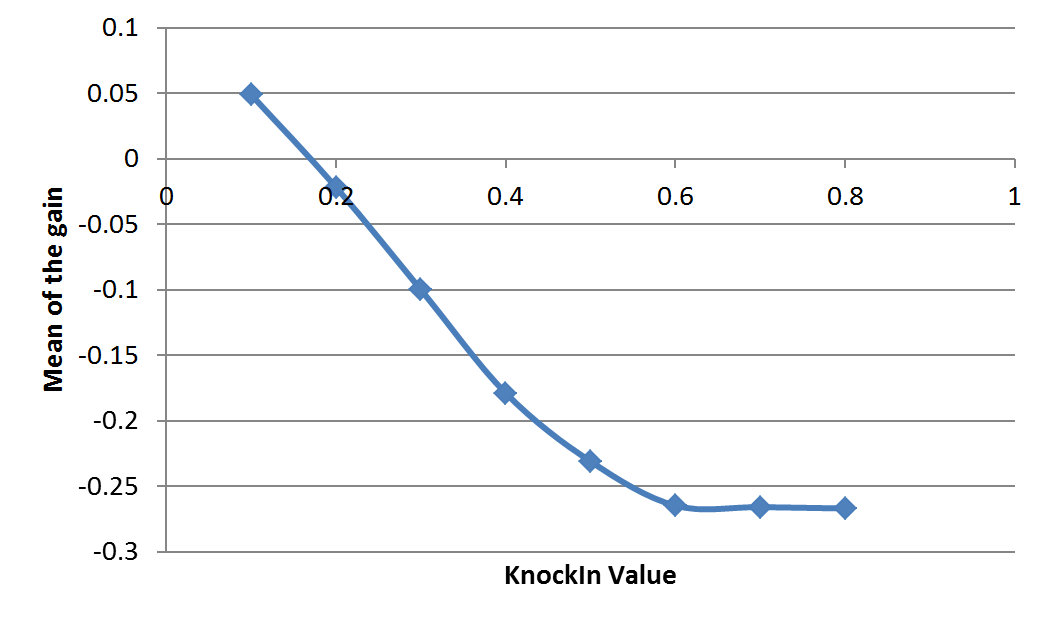
\includegraphics[width=7cm]{Mean_depending_on_knockin}
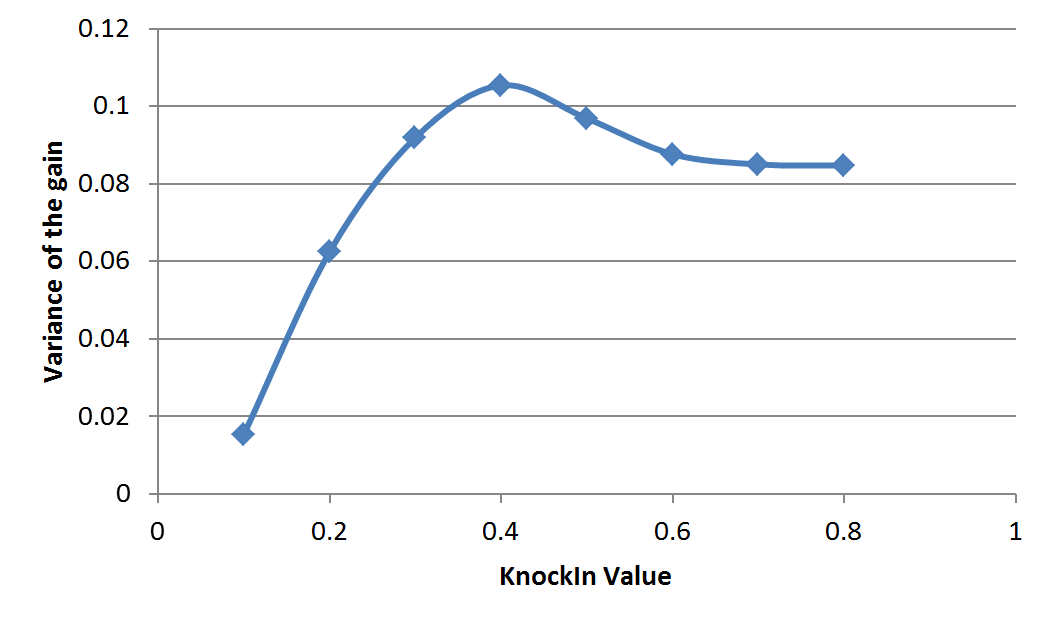
\includegraphics[width=7cm]{Variance_depending_on_knockin}
\caption{Mean (left) and variance (right) of the return depending on the knock-in value}
\end{figure}

As we can see on these graphs, to make the product fair, the knock-in value should be really low (approximately 20\%). It is, of course, impossible for a market price to reach such a low value except in case of crisis. We have also compared the cumulative density function of the return for the 60\% knock-in value and a 30\% knock-in value.

\begin{figure}[h!]
\centering
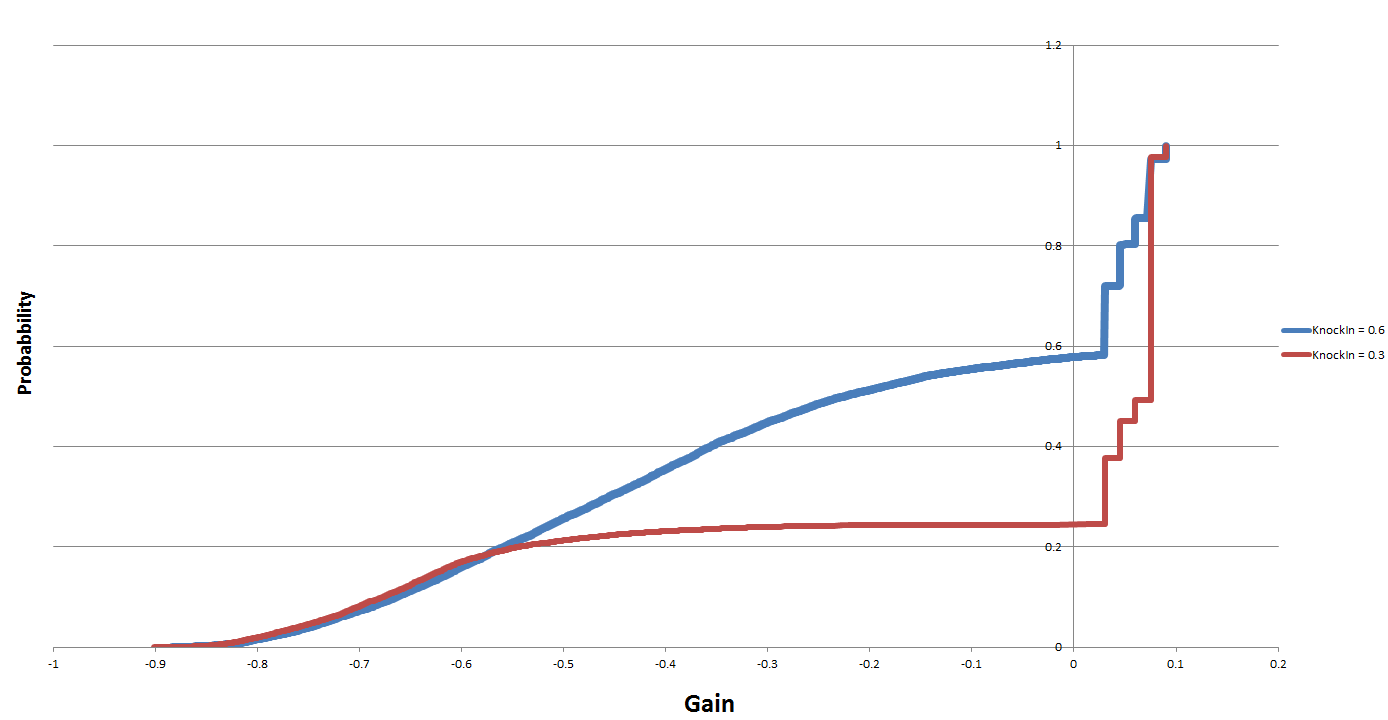
\includegraphics[width=12cm]{KnockInCDFComparaison}
\caption{Comparison of the CDF for knock-in value = 60\% (blue) and 30\% (red)}
\end{figure}

Of course, for a value of 30\% the maximum gain is not change but the probability to have a positive gain is clearly increased.

\end{document}